\documentclass{article}
\usepackage[utf8]{inputenc}

\title{CS 440 Summer \\ Project 2}
\author{Benjamin Pasternak, Junxian Cai}
\date{August 2020}

\usepackage{natbib}
\usepackage{graphicx}
\usepackage{pgfplots}
\usepackage{tikz,tikz-qtree} 
\usepackage{changepage}
\usepackage{amsmath}
\usetikzlibrary{backgrounds}

\newcommand{\ply}[3][black]{\footnotesize{#2 ({\color{#1}#3})}}
\newcommand{\plyy}[1]{\footnotesize{#1}}
\newcommand{\player}[1]{\footnotesize \emph #1}

\begin{document}

\maketitle

\section*{Algorithm description: Naive Bayes}
\paragraph*{}
Naive Bayes is a probabilistic classifier that relies on a few assumptions. Let $X = (X_1,X_2,\cdots , X_k)$ which represents $k$ features. $Y$ is the label with $K$ possible class values. $X_i \in X$ and $Y$ are random variables where the value of $X_i$ is $x$ and $Y\text{ is } y$. In order to make classifications, we need to use $X$ in order to predict $Y$. So if we are given data point $X = (x_1,x_2,\cdots ,x_n)$, we must find the odds that $Y=y$. Another important supposition of this method is that all conditional probabilities are independent of one another.\\

$$\text{(*) }P(Y=y\mid X = (x_1,x_2,\cdots ,x_n))$$\\
$$\text{predicted y = } argmax_yP((Y=y\mid X = (x_1,x_2,\cdots ,x_n))$$\\
\\
This result is the ultimate goal of the Naive Bayes classifier. However, in order to find this output we must use Bayes rule which is as follows. \\
\\
$$P(Y\mid X)=\frac{P(X\mid Y)P(Y)}{P(X)}$$
This must then be generalized to the following in order to work on k features:\\
$$P(Y\mid X_1,X_2,\cdots ,X_n)) = \frac{P(X_1,X_2,\cdots ,X_k\mid Y)P(Y)}{P(X_1,X_2,\cdots ,X_k)}$$
Since we can assume probabilities are independent:
$$= \frac{P(Y)\prod_{j=1}^{k} P(X_j\mid Y)}{P(X_1,X_2,\cdots ,X_k)}$$
Thus the generalized formula for $(*)$ is as follows:
$$\Vec{y} = argmax_{y_i}\prod_{j=1}^{k} P(X_j = x_j\mid Y = y_j)$$
I have read (Bengio, et. al.), that this problem is well modeled using the gaussian distribution. This follows the following assumptions. $P(X_j = x_j\mid Y = y_j)$ has a normal distribution with mean $\mu_{ij}$ and variance $\sigma_{ij}$. This of course means that $X_j$ are continuous random variables, however, $Y$ is a descrete random variable corresponding to the labels 0-9.\\
\\
Thus the probability density function is described as follows: $$P(X_j = x_j\mid Y = y_j) = f(x_j,\mu_{ij},\sigma_{ij}) = \frac{1}{\sigma_{ij}\sqrt{2\pi}}e^{-\frac{(x-\mu_{ij})^2}{2(\sigma_{ij})^2}}$$

Thus the final predictive model is as follows:\\
$$\Vec{y} = argmax_{y_i}P(Y=y_i)\prod_{j=1}^{k} f(x_j,\mu_{ij},\sigma_{ij})$$

\section*{Algorithm description: Perceptron}
\paragraph*{}
Perceptron is a simple nerual network with just one layer. The objective of the perceptron model is to learn a linear decision model defined as $f(x_i,w)=w_0+w_1\phi_1(x_i)+w_2\phi_2(x_i)+ \cdots + +w_k\phi_k(x_i)$\\
This formula is better defined as: 
$$f(x_i,w)=w_0+\sum_{j=1}^{k} w_j\phi_j(x_i)$$

This model, for a new test point $x$ predicts that label y = $true$ in the general case if $f(x_i,w)\geq 0$ and $f(x_i,w)\leq 0$.\\
\\
In our code, however, since we are not trying to receive an output of $true$ or $false$ from our perceptron, our update step, we find the max of $f(x_i,w)$ in training. If the predicted label is different from the actual label, we increase $f(x_i,w)$ of the actual label and decrease the falsely predicted label. 


\section*{Feature collection: Face Detection}
\paragraph*{}
For simple face detection we have only one general feature type which is collected in $easy\_face\_features()$ function. This function computes how many points in each row and column of the data array are relevant. This creates a robust feature which yields high accuracy. It is visualized below:\\
\bigskip{}

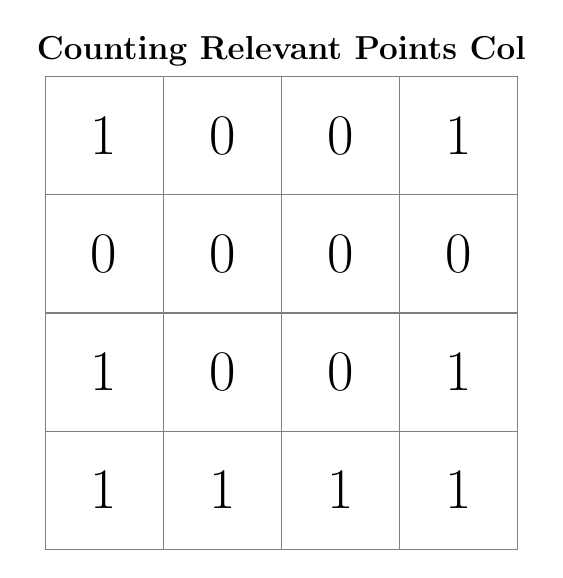
\begin{tikzpicture}
\draw[step=0.5cm,color=gray,xscale = 3,yscale = 3] (-1,-1) grid (1,1);
\node at (-2.25,+2.25) {\huge $1$}; %0,0
\node at (-0.75,+0.75) {\huge $0$};%1,1
\node at (+0.75,-0.75) {\huge $0$};%2,2
\node at (+2.25,-2.25) {\huge $1$};%3,3
\node at (-0.75,+2.25) {\huge $0$};%0,1
\node at (+0.75,+2.25) {\huge $0$};%0,2
\node at (+2.25,+2.25) {\huge $1$};%0,3
\node at (-2.25,+0.75) {\huge $0$};%1,0
\node at (+0.75,+0.75) {\huge $0$};%1,2
\node at (+2.25,+0.75) {\huge $0$};%1,3
\node at (+2.25,-0.75) {\huge $1$};%2,3
\node at (-0.75,-0.75) {\huge $0$};%2,1
\node at (-2.25,-0.75) {\huge $1$};%2,0
\node at (+0.75,-2.25) {\huge $1$};%3,2
\node at (-0.75,-2.25) {\huge $1$};%3,1
\node at (-2.25,-2.25) {\huge $1$};%3,0
\filldraw[draw=black,fill=white,opacity=0] (-3,3) rectangle (-1.5,-3);
\node[above,font=\large\bfseries] at (current bounding box.north) {Counting Relevant Points Col};
\end{tikzpicture}\\

For this row, we would count 3 relevant points in identifying smiling face. Thus we would have a value of 3 after counting this column. \\
\\
The same is also true for rows. 
Ultimately, we will have a feature vector that looks like [3,1,1,3,2,0,2,4]


\section*{Feature collection: Digit Detection}
\paragraph*{}
Feature detection includes the above feature detector function with a slight modification that accounts for the + and \# in digit representations. The difference, however is neglagable, instead of just counting the number of ones present, we count the number of ones and 2s present in each column and row and assemble the feature vector in this way. \\
\\
We do use another feature in digit recognition ($other\_feature()$), that is we count the number of 1s and 2s in each diagonal from the top left descending to the bottom right. This is again accumulated into a feature vector and is combined with the one described vide supra. 


\section*{Results of Work + Statistics}
\paragraph*{}
We repeated each test 5 times and have the following results:

\begin{figure}
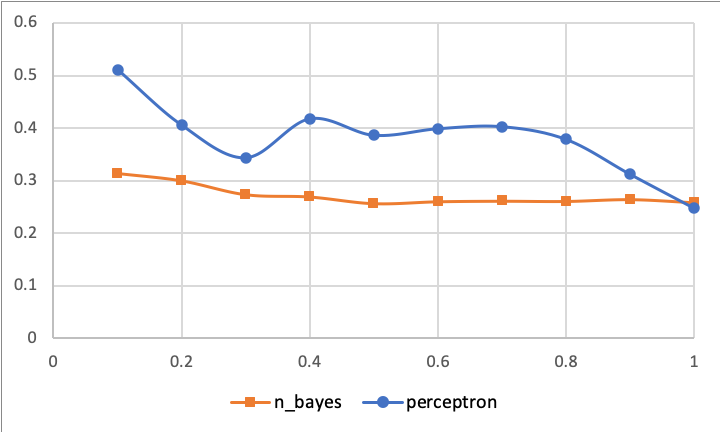
\includegraphics[width = 1\textwidth]{digit_error.png}
\caption{Classifying Digits Error}
\label{digit_error}
\end{figure}

\begin{figure}
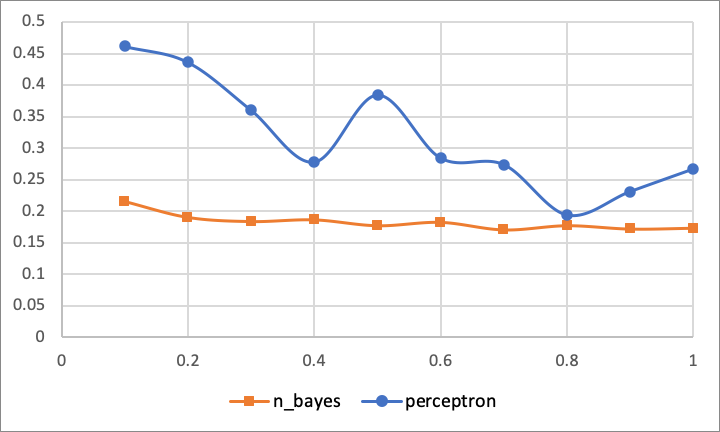
\includegraphics[width = 1\textwidth]{face_error.png}
\caption{Detecting Faces Error}
\label{face_error}
\end{figure}

\begin{figure}
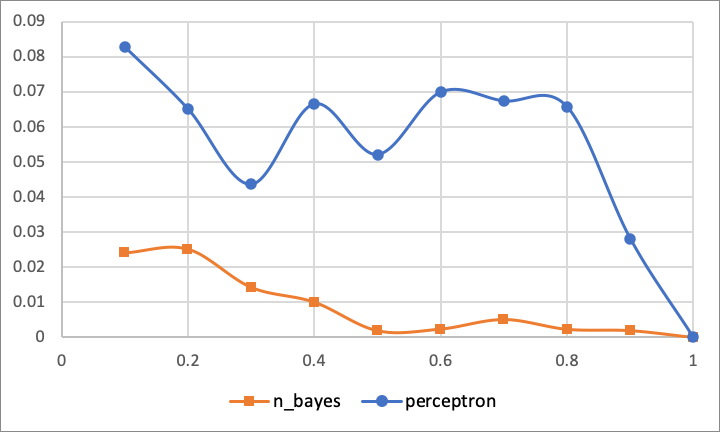
\includegraphics[width = 1\textwidth]{digit_std.png}
\caption{Classifying Digits Standard Deviation}
\label{digit_std}
\end{figure}

\begin{figure}
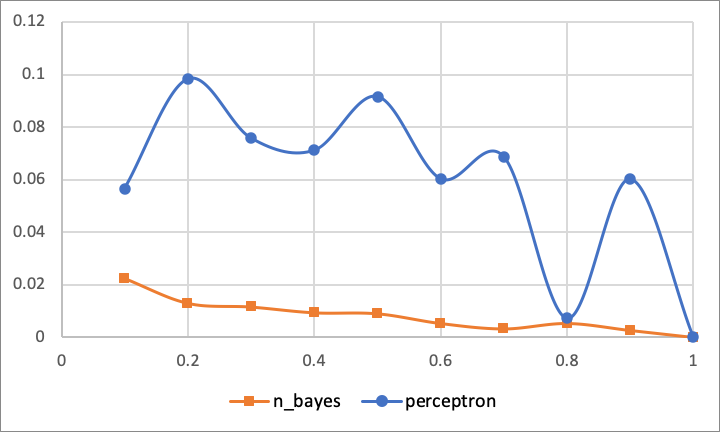
\includegraphics[width = 1\textwidth]{face_std.png}
\caption{Detecting Faces Standard Deviation}
\label{face_std}
\end{figure}

\begin{figure}
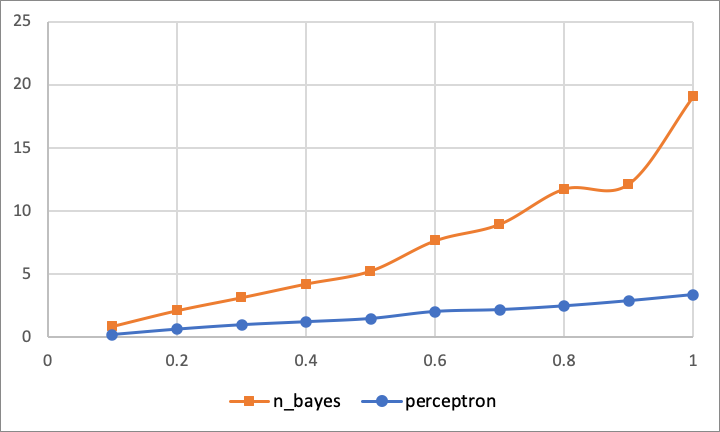
\includegraphics[width = 1\textwidth]{digit_time.png}
\caption{Classifying Digits Time Consumption}
\label{digit_time}
\end{figure}

\begin{figure}
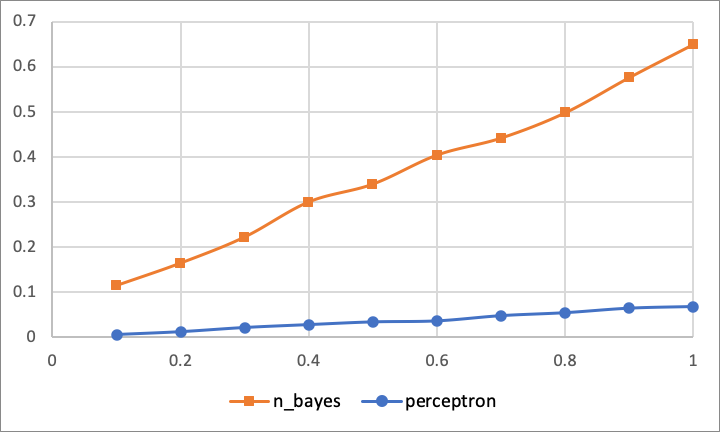
\includegraphics[width = 1\textwidth]{face_time.png}
\caption{Detecting Faces Time Consumption}
\label{face_time}
\end{figure}

\newpage
\paragraph*{}
From figure \ref{digit_error} and figure \ref{face_error} we can see Naive Bayes algorithm is more accurate than Perceptron using the same training data, and more stable as well by observing figure \ref{digit_std} and figure \ref{face_std}. But it took more time to train with the same set of data using Naive Bayes than Perceptron, as seen in figure \ref{digit_time} and figure \ref{face_time}.\\
In our Naive Bayes algorithm, $P$ is calculated with each feature that generalized with all data provided. But for Perceptron, $w_i$ are increased or decreased indiscriminately. This resulted in the higher accuracy and stability of Naive Bayes algorithm.\\
In terms of time consumption, Naive Bayes algorithm gathers every data to find the predictive model no matter if the model at some point is tested correct or not. For Perceptron algorithm, some training data will have no influence on the decision model if they match the model, hence spend less time than Naive Bayes algorithm.\\

\section*{Lesson Learned}
\paragraph*{}
We designed multiple features for both digit classification and facial recondition throughout the project, but usually the simple ones can better improve the accuracy. Some complicate features can even decrease the accuracy although we designed them specifically. The lesson we learned from this experience is that, rather than designing complex features with low distinguish ability, easy features that distinguishably different between classes are more useful. Generate more simple feature could be a better strategy than design a few complex feature.

\end{document}
